\documentclass{subfile}

\begin{document}
	\section*{Prologue}
	\large This booklet contains selected problems used in the training and selection process of the IMO team that participated in IMO $2015$. Many of the problems are taken from IMO Shortlisted problems. And many other are taken from other olympiads. We are grateful to the problem setters of those problems. They helped a lot in our training process. We hope it wouldn't raise any legal issue related to copyrights for using those problems since they were by no means used for any commercial gain. So we apologize in advance if it's any inconvenience for anyone. Also, thanks to anyone who contributed to the training process in any way, including our \textbf{MOVER}s(Math Olympiad Volunteers), who took care of the participants in the camp.
	
	I am very grateful to Mahi, Sanzeed, Asif and Swad for their time and contribution. At first, I wanted to create this document all by myself. But later I realized I don't have enough time for that. So, I invited Mahi. Later on I had to invite others too because we both got busy. Whereas it should have been published in $2015$, I couldn't do it until now. Therefore, it goes without saying that they had a lot to do with it.
	
	Another point I should mention is that, all problems may not have solution right now or some might contain typos. Probably in a later version, we will update it. If there are any typos or errors in solutions or any suggestions, feel free to email me: \url{billalmasum93@gmail.com}
	
	\begin{flushright}
		{\it Masum Billal}
	\end{flushright}
	\titlepage
	
	\begin{center}
		\begin{quote}
			\textbf{You can use this document in any form as long as you don't benefit commercially. Moreover, one of my primary motivations to create this document was to encourage other countries to publish their booklets as well. Because many countries tend to keep their training problems and materials secret. Therefore, you can share it as much as you want, and also enable others to share their booklet too.}
		\end{quote}
	\end{center}\newpage
	\section*{Bangladesh Mathematical Olympiad}
	In Bangladesh, students face at least twelve stages of primary, secondary and higher secondary education. Excluding pre-school studies, one has to study in classes $1-12$. Grades $1$ to $5$ are considered primary, $6-10$ secondary and $11-12$ is higher secondary. Mathematical competitions in Bangladesh are divided into four categories:
	\begin{enumerate}
		\item \textbf{Primary} Students of class $1-5$.
		\item \textbf{Junior} Students of class $6-8$.
		\item \textbf{Secondary} Students of class $9-10$.
		\item \textbf{Higher Secondary} Students of class $11-12$.
	\end{enumerate}
	It is to be noted that, we treat the participants of secondary and higher secondary category almost equally. Therefore, most problems posed for these two categories are about same.
	
	Two contests are held: one on a regional level and the other on a national level. At first, regional contests are held in different districts, $21$ this year. In a district, a school provides the venue of the regional olympiad. Participants who are awarded gets to participate in the national olympiad. The olympiads take place in a festive manner and the national level olympiad is known as \textbf{BdMO}(Bangladesh Mathematical Olympiad). Around $40$ participants are chosen as campers of the \textit{national math camp}, where some exams are held in order to determine the team for the IMO. Sometimes, there is an extension camp, where around $20$ campers are called for in order to take part in mock exams of \textbf{Team Selection Tests}. Finally a pool of at most six students is selected to represent Bangladesh at the International Mathematical Olympiad.\newpage
	
	\begin{center}
		\begin{figure}
			\centering
			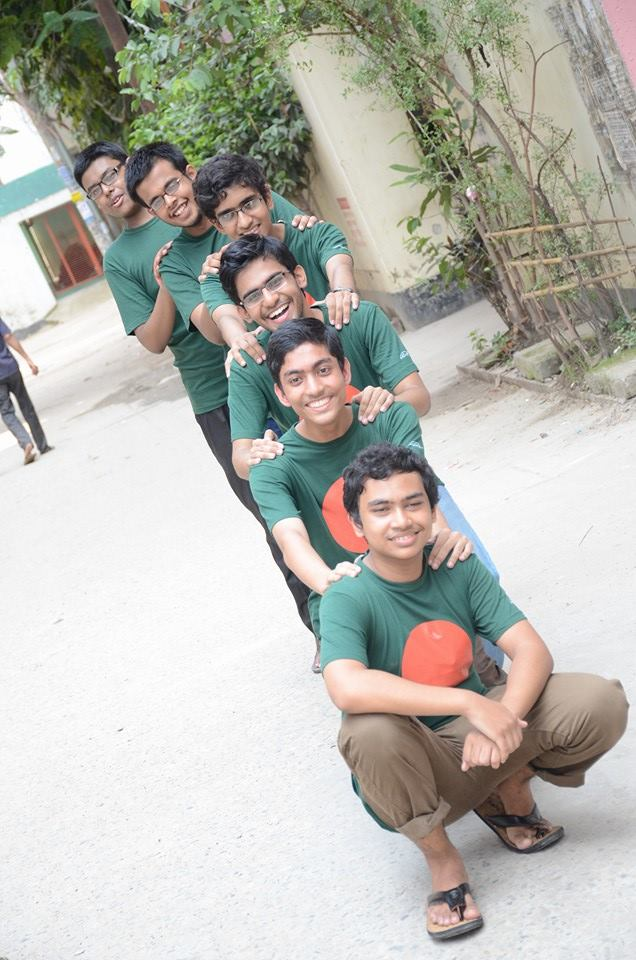
\includegraphics[scale=.6]{imoteam}
			\caption{Bangladesh IMO Team 2015, at the IMO Camp}
			\label{fig:imoteam}
		\end{figure}
	\end{center}
	\section*{IMO Contestants of $2015$}
	From right to left in figure \eqref{fig:imoteam}, the members are:
	\begin{itemize}
		\item Asif E Elahi\\ \textit {2015 Bronze, 2014 HM}
		\item Nayeemul Islam Swad\\ \textit { 2015 HM}
		\item Adib Hasan\\ \textit {2015, 14, 13 Bronze, 2012 HM}
		\item Sazid Akhter Turzo\\ \textit {2015 Bronze, 2014 HM}
		\item Sanzeed Anwar\\ \textit {2015 Silver, 2014 HM}
		\item Sabbir Rahman Abir\\ \textit {2015 Bronze}
	\end{itemize}
	
	\newpage
	\section*{Trainer Panel of $2015$}
	This year the following trainers contributed in the math camps by taking classes and setting problemsets.
	
	\begin{enumerate}
		\item Dr. Mahbub Majumdar (coach of BdMO and leader of our IMO team)
		\item Masum Billal
		\item Nur Muhammad Shafiullah
	\end{enumerate}
	Special thanks to Muhammad Milon(A BIG THANK YOU to him. He cheered up and entertained everyone throughout his classes when all the campers were in the ICU called national math camp) and Zadid Hasan.
	\tableofcontents
	
	\chapter*{Notations}
	
	\begin{itemize}
		\item $a$ divides $b$ is denoted by $a|b$
		\item $(a,b)=\gcd(a,b)$ is the greatest common divisor of $a$ and $b$.
		\item $[a,b]=\lcm(a,b)$ is the least common multiple of $a$ and $b$.
		\item $\tau(a)$ is the number of divisors of $a$.
		\item $\s (n)$ is the sum of divisors of $n$.
		\item $\t (n)$ is the number of positive integers less than or equal to $n$ which are co-prime to $n$.
		\item $\pi(n)$ is the number of primes less than or equal to $n$.
		\item $\nu_p(n)=\a$ is the largest positive integer so that $p^\a|n$ but $p^\a\not|n$.
		\item $\L(n)$ is the \textit{Van Mangoldt Function}.
	\end{itemize}
\end{document}